\documentclass{standalone}
\usepackage{tikz}
\begin{document}
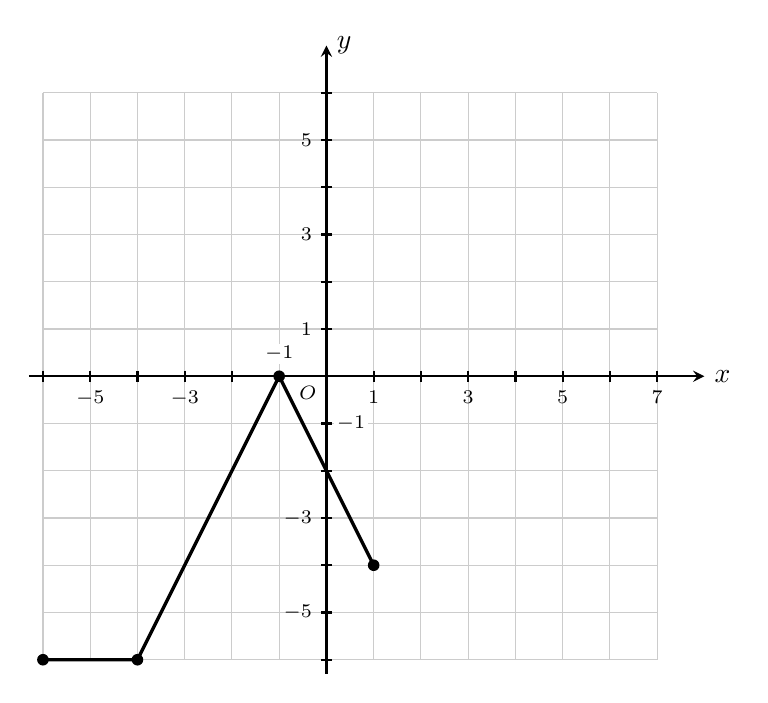
\begin{tikzpicture}[color=black, >=stealth, scale=0.6]
  % Grid: x from -6 to 7, y from -6 to 6
  \draw[gray!40, thin] (-6,-6) grid (7,6);
  % Axes (left and bottom ends run just past the grid with no arrowhead)
  \draw[->, thick] (-6.3,0) -- (8,0) node[right] {$x$};
  \draw[->, thick] (0,-6.3) -- (0,7) node[right] {$y$};
  % Tick marks at every integer
  \foreach \x in {-6,...,7} \draw[thick] (\x,0.12) -- (\x,-0.12);
  \foreach \y in {-6,...,6} \draw[thick] (0.12,\y) -- (-0.12,\y);
  % Tick labels at odd values only
  \foreach \x in {-5,-3,1,3,5,7} \node[font=\scriptsize, below] at (\x,-0.1) {$\x$};
  \foreach \y in {-5,-3,1,3,5} \node[font=\scriptsize, left] at (-0.1,\y) {$\y$};
  % The two -1 labels are moved off the graph segments (above the x-axis, right of the y-axis)
  \node[font=\scriptsize, above, fill=white, inner sep=1pt] at (-1,0.25) {$-1$};
  \node[font=\scriptsize, right, fill=white, inner sep=1pt] at (0.15,-1) {$-1$};
  \node[font=\scriptsize, below left] at (0,0) {$O$};
  % Piecewise-linear graph: (-6,-6)--(-4,-6)--(-1,0)--(1,-4)
  \draw[line width=1.2pt] (-6,-6) -- (-4,-6) -- (-1,0) -- (1,-4);
  % Filled endpoints and vertices
  \foreach \p in {(-6,-6),(-4,-6),(-1,0),(1,-4)} \fill[black] \p circle (3.5pt);
\end{tikzpicture}
\end{document}
